\scanpage{397}
Je m'intéresse surtout à l'hom. induit
\[
 (4)\qquad
 \diagram{\begin{tikzcd}[ampersand replacement=\&]
 \deleted{\unsure{\mathcal A}}\mathcal{M}_{\rho,\sigma}
 \arrow[r,"\Theta"] \& G\simeq\mathrm{Gl}(2)_S
 \end{tikzcd}}
\]
il est \unsure{évidemt} épi, car son image contient
\unsure{trivial\textsuperscript{mt}} $SG$, donc il suffit de voir
que le composé avec
\[
 \diagram{\begin{tikzcd}[ampersand replacement=\&]
 G/SG\arrow[r,"\det","\sim"'] \& \mathbb G_m
 \end{tikzcd}}
\]
est épi, i.e. que le composé avec $\det$ l'est,
or ce composé est aussi l'hom (noté encore $\chi$)
\[
 (5)\qquad
 \diagram{\begin{tikzcd}[ampersand replacement=\&,column sep=large]
 \mathcal{M}_{\rho,\sigma}
 \arrow[r,"\substack{\text{projection}\\\text{canonique}}"]
 \arrow[d,phantom,"\rotatebox{90}{$\simeq$}"]
 \& S\mathcal{G}_{\rho,\sigma}^{*\unsure{\flat|\sharp}}(0)
 \deleted{\unsure{\infty}}
 \arrow[r,"\text{multiplicateur}"] \& \mathbb G_m \\
 S\mathcal{G}_{\rho,\sigma}^{*\unsure{\flat|\sharp}}(0)\mathbin{.}SG
 \& (\alpha,\beta,\mu,\varepsilon)\arrow[r,mapsto] \& \mu
 \end{tikzcd}}
\]
qui est épi --- en termes de
\[
 (6)\qquad
 \diagram{\begin{tikzcd}[ampersand replacement=\&]
 S\mathcal{G}_{\rho,\sigma}^{*\unsure{\flat|\sharp}}(0)
 \arrow[r,hook] \& \deleted{\unsure{\mathbb G_m}}T_0\times T_\rho\times N'_\sigma
 \end{tikzcd}}
\]
ce sera
\[
 \diagram{\begin{tikzcd}[ampersand replacement=\&]
 (\uline{u},\uline{a},\uline{b})\arrow[r,mapsto] \& \det\uline{u}
 \end{tikzcd}},
\]
en termes de
\[
 (7)\qquad
 \diagram{\begin{tikzcd}[ampersand replacement=\&]
 S\mathcal{G}_{\rho,\sigma}^{*\unsure{\flat|\sharp}}(0)
 \arrow[r,hook] \& T_\rho\times N'_\sigma
 \end{tikzcd}}
\]
ce sera
\[
 \diagram{\begin{tikzcd}[ampersand replacement=\&]
 (\uline{a},\uline{b})\arrow[r] \& \det\uline{b}
 \end{tikzcd}}
\]
(cf \uline{VIII}, p. 489 en particulier (25)).

Définissons
\[
 (8)\qquad
 \mathcal{M}_{\rho,\sigma}^{+}\overset{\text{déf}}{=}
 \operatorname{Ker}\left(
 \diagram{\begin{tikzcd}[ampersand replacement=\&]
 \mathcal{M}_{\rho,\sigma}\arrow[r,"\chi"] \& \mathbb G_m
 \end{tikzcd}}\right),
\]
on aura donc un hom de suites exactes
\margin{396}

\scanpage{398}
\mspage{500}
\[
 (9)\qquad
 \diagram{\begin{tikzcd}[ampersand replacement=\&,column sep=large,row sep=large]
 1\arrow[r,dash] \& \mathcal M_{\rho,\sigma}^{+}\arrow[r,dash]\arrow[d]
 \& \mathcal M_{\rho,\sigma}\arrow[r]\arrow[d,"\Theta"]
 \& \mathbb G_m\arrow[r]\arrow[d,"\deleted{\unsure{\det}}"] \& 1\\
 1\arrow[r] \& \deleted{\unsure{SLG}}SG\arrow[r,hook]
 \& G\arrow[r,"\det"] \& \mathbb G_m\arrow[r] \& 1
 \end{tikzcd}}
\]
qu'on rapprochera de §39 p. 299 (1)

Comme $\mathcal M_{\rho,\sigma}$ est plat de dim relative
6, et $G$ \unsure{idm|idem} de dim relative 4, le
noyau de l'épi $\Theta\colon\mathcal M_{\rho,\sigma}\longrightarrow G$ est
nécessairement plat de dim relative 2. \unsure{Notons}-le
$I_{\rho,\sigma}$, il est contenu dans le
noyau $J_{\rho,\sigma}$ (de dim relative 3)
du composé
\[
 \diagram{\begin{tikzcd}[ampersand replacement=\&]
 \mathcal M_{\rho,\sigma}\arrow[r]\&G\arrow[r]\&PG
 \end{tikzcd}},
\]
de sorte qu'on a
\[
 (10)\qquad
 \diagram{\begin{tikzcd}[ampersand replacement=\&]
 1\arrow[r,dash]\&I_{\rho,\sigma}\arrow[r]\&J_{\rho,\sigma}\arrow[r]
 \&\mathbb G_m\arrow[r]\&1\arrow[r,dash]\&\unsure{1}
 \end{tikzcd}}
\]
et une suite de composition de $\mathcal M_{\rho,\sigma}$
\[
 (11)\qquad
 \diagram{\begin{tikzcd}[ampersand replacement=\&,column sep=large,row sep=large]
 1\arrow[r,phantom,"\subset"]
 \& I_{\rho,\sigma}\arrow[r,phantom,"\subset"]
 \arrow[rr,dash,start anchor=south,end anchor=south,
 to path={-- ++(0,-1.1) -- node[below] {$G$} ([yshift=-1.1cm]\tikztotarget) -- (\tikztotarget)}]
 \& J_{\rho,\sigma}\arrow[r,phantom,"\subset"]
 \arrow[r,dash,start anchor=south,end anchor=south,
 to path={-- ++(0,-0.4) -- node[below] {$PG\simeq SG/\mu_2$} ([yshift=-0.4cm]\tikztotarget) -- (\tikztotarget)}]
 \&\mathcal M_{\rho,\sigma}
 \end{tikzcd}}
\]
Le groupe $J_{\rho,\sigma}$ joue le rôle d'un
\uline{radical} --- on prévoit qu'il est commutatif,
(de dim relative 3) --- et \inserted{à composantes}
\unsure{toriques|torique} si
\margin{397}

\scanpage{399}
$T_\rho^{\circ},T_\sigma^{\circ}$ sont des tores.

Mais je vois que je me complique
l'existence pour être trop savant dans mes
\unsure{déductions|directions}. En effet, par construction
du produit $\frac12$ direct, on a
\[
 \diagram{\begin{tikzcd}[ampersand replacement=\&,column sep=small,row sep=small]
 \mathcal M_{\rho,\sigma}=S\mathcal G_{\rho,\sigma}^{*}\mathbin{.}SG
 \arrow[r,hook,dash] \&(T_0\times T_\rho\times N'_\sigma)\mathbin{.}SG
 \arrow[d,phantom,"\rotatebox{90}{$\simeq$}"]\\
 \& (T_\rho\times N'_\sigma)\times\underbrace{(T_0\mathbin{.}SG)}_{G}
 \end{tikzcd}}
\]
ainsi
\[
 (12)\qquad
 \diagram{\begin{tikzcd}[ampersand replacement=\&,column sep=large,row sep=large]
 \mathcal M_{\rho,\sigma}\arrow[r,hook]\arrow[dr,"\Theta"']
 \&T_\rho\times N'_\sigma\times G\arrow[d,"\mathrm{pr}_3"]\\
 \&G
 \end{tikzcd}}
\]
d'ailleurs $\mathcal M_{\rho,\sigma}$ est défini dans ce
produit par les conditions
\[
 (13)\qquad
 \begin{aligned}
 \mathcal M_{\rho,\sigma}&\subset T_\rho\times N'_\sigma\times G\\
 &\simeq\{(x,y,f)\mid\det f=\det y=\varepsilon'\det x,\quad
 \varepsilon'^2=1\}
 \end{aligned}
\]
Cela montre que
\[
 (14)\qquad
 \begin{aligned}
 \deleted{\unsure{J}}I_{\rho,\sigma}
 &\hookrightarrow T_\rho\times N'_\sigma\times\mathbb G_m\\
 &\simeq\{(x,y,\lambda)\mid
 \det\deleted{\unsure{x}}y=\deleted{\det}\varepsilon\det x=\lambda^2,
 \quad\varepsilon^2=1\}\\[1em]
 \unsure{J|I}_{\rho,\unsure{\sigma|x}}
 &\subset T_\rho\times N_\sigma^{\prime\unsure{\flat|\sharp}}\\
 &\simeq\{(x,y)\mid\det y=1,\ (\det x)^2=1\}
 \end{aligned}
\]
Il me semble plus naturel de
faire le \unsure{dévissage} de $\mathcal M_{\rho,\sigma}$ en commençant
par descendre à la composante neutre $\mathcal M_{\rho,\sigma}^{\circ}$,
\margin{398}

\scanpage{400}
\mspage{501}
le groupe
\[
 (15)\qquad
 \diagram{\begin{tikzcd}[ampersand replacement=\&,column sep=small,row sep=tiny]
 \inserted{\text{\unsure{compos.} neutre}}\arrow[d,dash]\!\&\\[-0.3em]
 \mathcal M_{\rho,\sigma}/\mathcal M_{\rho,\sigma}^{\circ}
 \arrow[r,phantom,"\simeq"]
 \&\mathcal G_{\rho,\sigma}^{*}(0)/\mathcal G_{\rho,\sigma}^{*}(0)^{\circ}
 \simeq\mu_2\times\mu_2
 \end{tikzcd}}
\]
(cf p. 489 (23)), on aura donc
\[
 \diagram{\begin{tikzcd}[ampersand replacement=\&,column sep=small,row sep=small]
 \mathcal M_{\rho,\sigma}^{\circ}=\mathcal G_{\rho,\sigma}^{*}(0)^{\circ}\mathbin{.}SG
 \arrow[r,hook,dash]
 \&(T_0\times T_\rho\times T_\sigma)\mathbin{.}SG
 \arrow[d,phantom,"\rotatebox{90}{$\simeq$}"]\\
 \&T_\rho\times T_\sigma\times
 \underbrace{(T_0\mathbin{.}SG)}_{\substack{\simeq\\G}}
 \arrow[d,phantom,"\rotatebox{90}{$\simeq$}"]\\
 \&T_\rho\times T_{\unsure{\sigma|\rho}}\times G
 \end{tikzcd}}
\]
\[
 (16)\qquad
 \begin{aligned}
 \mathcal M_{\rho,\sigma}^{\circ}&\lhook\joinrel\longrightarrow
 T_\rho\times T_\sigma\times G\\
 &\simeq\left\{
 \left(\underset{\substack{\rotatebox{90}{$\in$}\\\Gamma T_\rho}}{x},
 \underset{\substack{\rotatebox{90}{$\in$}\\\Gamma T_\sigma}}{y},
 \underset{\substack{\rotatebox{90}{$\in$}\\\Gamma G}}{f}\right)
 \mathrel{\Big|}\det x=\det y=\det f\right\}
 \end{aligned}
\]
Donc le noyau
\[
 (17)\qquad\left\{
 \begin{aligned}
 J_{\rho,\sigma}^{\circ}&\overset{\text{déf}}{=}
 \operatorname{Ker}\left(
 \diagram{\begin{tikzcd}[ampersand replacement=\&,row sep=tiny]
 \mathcal M_{\rho,\sigma}^{\circ}\arrow[r]\&PG
 \arrow[d,phantom,"\rotatebox{90}{$\simeq$}"]\\
 \&G/\mathbb G_m
 \end{tikzcd}}\right)\\
 &\simeq\left\{
 \left(\underset{\substack{\rotatebox{90}{$\in$}\\\Gamma T_\rho}}{x},
 \underset{\substack{\rotatebox{90}{$\in$}\\\Gamma T_\sigma}}{y},
 \underset{\substack{\rotatebox{90}{$\in$}\\\Gamma\mathbb G_m}}{\lambda}\right)
 \mathrel{\Big|}\det x=\det y=\unsure{\lambda^2}\right\}
 \deleted{\unsure{\simeq T_\rho\times_{\mathbb G_m}T_\sigma}}\\[0.6em]
 &\simeq T_\rho\times_{\mathbb G_m}T_\sigma
 =\{(x,y)\mid\det x=\det y\}\\
 &\simeq S\mathcal G_{\rho,\sigma}^{\unsure{*}}(0)^{\circ}
 \end{aligned}\right.
\]
Enfin, on en déduit que
\[
 (18)\qquad
 \begin{aligned}
 I_{\rho,\sigma}^{\circ}&\overset{\text{déf}}{=}
 \operatorname{Ker}\left(
 \diagram{\begin{tikzcd}[ampersand replacement=\&]
 \mathcal M_{\rho,\sigma}^{\circ}\arrow[r]\&G
 \end{tikzcd}}\right)\\
 &\simeq ST_\rho\times ST_\sigma
 =\left\{\left(
 \underset{\substack{\rotatebox{90}{$\in$}\\\Gamma T_\rho}}{x},
 \underset{\substack{\rotatebox{90}{$\in$}\\\Gamma T_\sigma}}{y}
 \right)\mathrel{\Big|}\det x=\det y=1\right\}.
 \end{aligned}
\]
Récapitulons :
\margin{399}

\scanpage{401}
\uline{Théorème} Le groupe
\[
 (19)\qquad
 \diagram{\begin{tikzcd}[ampersand replacement=\&,column sep=small,row sep=small]
 \mathcal M_{\rho,\sigma}\arrow[r,phantom,"{\overset{\text{déf}}{\simeq}}"]
 \&\mathcal G_{\rho,\sigma}^{*}(0)\mathbin{.}SG
 \arrow[d,phantom,"\rotatebox{90}{$\subset$}"]
 \&\inserted{\text{cf définition p. 487' (20)}}\arrow[l]\\
 \&T_0\times T_\rho\times N'_\sigma\&
 \end{tikzcd}}
\]
est extension de $\mu_2\times\mu_2$ par $\mathcal M_{\rho,\sigma}^{\circ}$
\[
 (20)\qquad
 \diagram{\begin{tikzcd}[ampersand replacement=\&]
 1\arrow[r]\&\mathcal M_{\rho,\sigma}^{\circ}\arrow[r,dash]
 \&\mathcal M_{\rho,\sigma}\arrow[r]\&\mu_2\times\mu_2\arrow[r]\&1
 \end{tikzcd}}.
\]
\inserted{déduit de
\[
 \diagram{\begin{tikzcd}[ampersand replacement=\&]
 \mathcal G_{\rho,\sigma}^{*}\deleted{\unsure{(0)}}\arrow[r]\&\mu_2\times\mu_2\\
 \deleted{(\alpha,\beta,\mu,\varepsilon)}\ (\alpha,\beta,\mu,\varepsilon)
 \arrow[r]\&(\det\alpha,\varepsilon(=\det\uline b))
 \end{tikzcd}}
\]}
Dans $\mathcal M_{\rho,\sigma}^{\circ}$ \unsure{on}
\deleted{\unsure{a deux}}\inserted{le} sous-groupe
\deleted{remarquables : le sous-groupe} \uline{central}
(dans $\mathcal M_{\rho,\sigma}$ tout entier)
\[
 (21)\qquad
 \diagram{\begin{tikzcd}[ampersand replacement=\&]
 ST_\rho\times ST_\sigma\arrow[r,hook]
 \&\mathcal G_{\rho,\sigma}^{*}(0)\arrow[r,hook]
 \&\mathcal M_{\rho,\sigma}
 \end{tikzcd}},
\]
et une suite exacte
\[
 \deleted{\unsure{(22)}}\quad\unsure{(21)|(22)}\qquad
 \diagram{\begin{tikzcd}[ampersand replacement=\&,row sep=large]
 1\arrow[r]\arrow[rrrr,dash,start anchor=north west,end anchor=south east,
 to path={([xshift=-3mm,yshift=5mm]\tikztostart) rectangle
 ([xshift=3mm,yshift=-5mm]\tikztotarget)}]
 \&ST_\rho\times ST_\sigma\arrow[r]\&\mathcal M_{\rho,\sigma}^{\circ}
 \arrow[r,"\Theta"]\&G\arrow[r]\&1\\
 \&\&\inserted{SG}\arrow[u,hook]\&\&
 \end{tikzcd}}
\]
On a \deleted{\unsure{donc}} dans $\mathcal M_{\rho,\sigma}^{\circ}$
une \deleted{suite de composition}\inserted{structure d'\unsure{extension}}
\[
 \diagram{\begin{tikzcd}[ampersand replacement=\&,row sep=large]
 \deleted{1\subset ST_\rho\times ST_\sigma\times SG
 \subset J_{\rho,\sigma}^{\circ}\unsure{\times|\mathbin{.}}SG}\\
 \inserted{\begin{gathered}
 \text{\uline{NB}}\\
 J_{\rho,\sigma}^{\circ}\text{ est encore}\\
 \text{central dans }\mathcal M_{\rho,\sigma}\\
 \text{et }J_{\rho,\sigma}^{\circ}\cap SG\simeq
 \end{gathered}}
 \arrow[u,bend left=15]\arrow[u,bend right=20]
 \end{tikzcd}}
\]
\[
 (23)\qquad
 \diagram{\begin{tikzcd}[ampersand replacement=\&,row sep=small]
 \&\&x\arrow[r,mapsto]\&\chi(x),\varepsilon(x),\varepsilon'(x)\&\\
 1\arrow[r]\arrow[rrrr,dash,start anchor=north west,end anchor=south east,
 to path={([xshift=-3mm,yshift=5mm]\tikztostart) rectangle
 ([xshift=3mm,yshift=-5mm]\tikztotarget)}]
 \&ST_\rho\times ST_\sigma\times SG\arrow[r]
 \&\mathcal M_{\rho,\sigma}\arrow[r]\&\mathbb G_m\times\mu_2\times\mu_2\arrow[r]\&1
 \end{tikzcd}}
\]
i.e.
\[
 (24)\qquad
 \mathcal M_{\rho,\sigma}^{\circ+}\simeq ST_\rho\times ST_\sigma\times SG\unsure{\}}
\]
\deleted{et on a aussi (\unsure{utilisant} l'inclusion
$(G\longrightarrow\mathcal M_{\rho,\sigma}^{\circ})$)}
\inserted{\unsure{inexistant}}
\[
 \diagram{\begin{tikzcd}[ampersand replacement=\&]
 \deleted{ST_\rho\times ST_\sigma\times G}
 \arrow[r,"\deleted{\unsure{\longrightarrow}}",phantom]
 \&\deleted{\mathcal M_{\rho,\sigma}^{\circ}}
 \arrow[r,"\deleted{\longrightarrow}",phantom]\&\deleted{1}
 \end{tikzcd}}
\]
On a un hom. canonique
\[
 (25)\qquad
 \diagram{\begin{tikzcd}[ampersand replacement=\&,column sep=small,row sep=small]
 \mu_2\times\mu_2\times\mu_2\arrow[r,hook]
 \&\mathcal M_{\rho,\sigma}^{\circ+}
 \overset{\text{déf}}{=}\operatorname{Ker}
 (\mathcal M_{\rho,\sigma}^{\circ}\overset{\chi}{\longrightarrow}\mathbb G_m)
 \arrow[d,phantom,"{\rotatebox{90}{$\simeq$}\ (24)}"]\\
 \&ST_\rho\times ST_\sigma\times SG
 \end{tikzcd}}
\]
\margin{400}

\scanpage{402}
\mspage{502}

grâce aux inclusions canoniques
\[
\tag{26}
\mu_2\subset ST_\rho,\qquad
\mu_2\subset ST_\sigma,\qquad
\mu_2\subset SG
\]
donnant naissance à des hom. canoniques déjà \unsure{envisagés} par ailleurs
\[
\tag{27}
\Sigma=(\mathbb Z/2\mathbb Z)^3\longrightarrow
\Gamma\mathcal M_{\rho,\sigma}^{\circ+}\deleted{\unsure{+}}
\subset\Gamma\mathcal M_{\rho,\sigma}^{\unsure{+|*}}.
\]

Je vais introduire au sujet du groupe $\mathcal M_{\rho,\sigma}$ des notations qui paraphrasent les notations $\mathcal M_{0,3}$ etc, dans le contexte des schémas en groupes. Le sous-groupe invariant $SG$ de $\mathcal M_{\rho,\sigma}$ sera aussi noté $\widetilde G_{\rho,\sigma}^{+}$ (l'analogue de $\widehat{\widetilde G}_{0,3}^{+}$), le quotient
\[
\tag{28}
\deleted{\unsure{\mathcal M}}
\mathcal M_{\rho,\sigma}/\widetilde G_{\rho,\sigma}^{+}
\simeq\tau_{\rho,\sigma}^{!}
\]
\unsure{paraphrase} $\tau_{0,3}^{!}$, on a d'ailleurs
\[
\tag{29}
\tau_{\rho,\sigma}^{!}\simeq S\mathcal G_{\rho,\sigma}^{*}(0)
\hookrightarrow T_0\times T_\rho\times N'_\sigma
\]
\margin{\unsure{Vu un peu traîner} le signe $!$, (\deleted{\unsure{qui}} $(28)$ \unsure{est tombé au loin} --- \unsure{même dans la suite suivant I}) c'est $\Gamma_{\rho,\sigma}$ (et non $\tau_{\rho,\sigma}$ \unsure{dans l'expression !}) qu'il conviendrait de \unsure{noter} ce groupe !}

--- par la suite la notation plus simple et plus suggestive $\tau_{\rho,\sigma}$ sera utilisée de préférence à $S\mathcal G_{\rho,\sigma}^{*}(0)$. On a donc
\[
\tag{30}
\diagram{\begin{tikzcd}[ampersand replacement=\&,column sep=small]
1\arrow[r]\&\widetilde G_{\rho,\sigma}^{+}\arrow[r]\arrow[d,phantom,"\rotatebox{90}{$\simeq$}"]\&\mathcal M_{\rho,\sigma}\arrow[r]\&\tau_{\rho,\sigma}^{!}\arrow[r]\&1\\
\&SG\simeq\mathrm{Sl}(2)_S\&\&\&
\end{tikzcd}}
\]
et un scindage canonique en produit semi-direct
\[
\tag{31}
\mathcal M_{\rho,\sigma}\simeq\mathcal M_{\rho,\sigma}(0)\mathbin{.}\widetilde G_{\rho,\sigma}^{+}
\]
\margin{401}

\scanpage{403}

où
\[
\tag{32}
\diagram{\begin{tikzcd}[ampersand replacement=\&]
\mathcal M_{\rho,\sigma}(0)\arrow[r,hook]\arrow[dr,"\sim"']\&\mathcal M_{\rho,\sigma}\arrow[d,"\mathrm{can}"]\\
\&\tau_{\rho,\sigma}^{!}
\end{tikzcd}}
\]
est un sous-groupe isomorphe à $\tau_{\rho,\sigma}^{!}$ --- qui correspond au sous-groupe $\mathcal M_{0,3}^{!\sim}(0)$ dans $\mathcal M_{0,3}^{\sim}$ ($\S\unsure{45|46}$, $\uline{\mathrm V}$).

\uline{Rmq.} On aurait envie d'introduire un $\tau_{\rho,\sigma}$ extension \inserted{(ou produit)} de $\tau_{\rho,\sigma}^{!}$ par un groupe tel que $\widetilde G_3$ (qui serait noté $\tau_{\rho,\sigma}^{+}$), en relation avec un sous-groupe $\pi_{\rho,\sigma}$ de $\widetilde G_{\rho,\sigma}^{+}$ \deleted{qui} tel que $\widetilde G_{\rho,\sigma}^{+}/\pi_{\rho,\sigma}\simeq\widetilde G_3$ --- mais ce n'est pas possible dans le contexte des \uline{schémas} en groupes ($\overline{\mathrm m}$ dans le cas particulier modulaire), vu que $\widetilde G_{\rho,\sigma}^{+}\simeq\mathrm{Sl}(2)_S$ est \unsure{connexe} \unsure{relativement} sur $S$. Par contre on peut, dans le ``cas modulaire'' $\rho=\begin{pmatrix}0&1\\-1&1\end{pmatrix}$, $\sigma=\begin{pmatrix}0&1\\-1&0\end{pmatrix}$ introduire une section canonique
\[
\tag{33}
\unsure{\dot\tau|\dot t}=\unsure{\dot\tau_\infty|\dot t_\infty}\in\Gamma(\tau_{\rho,\sigma}^{!})
\]
dont le représentant $\tau_\infty$ dans $\Gamma\unsure{\mathcal M}_{\rho,\sigma}^{!}(0)$ s'explicite comme
\[
\tag{34}
\tau_\infty=\begin{pmatrix}-1&0\\0&+1\end{pmatrix}.
\]

(Il serait intéressant de voir si, en dehors du
\margin{402}

\scanpage{404}
\mspage{503}

cas modulaire, on peut introduire des ``anti-involutions'' qui généralisent les réflexions géométriques
\[
\tag{35}
\left\{
\begin{aligned}
\deleted{\unsure{\tau}}r_0&=\tau'_\infty=\begin{pmatrix}0&1\\1&\unsure{0}\end{pmatrix}\\
r_1&=-\tau'_0=\begin{pmatrix}-1&1\\0&1\end{pmatrix}\\
r_\infty&=\tau_\infty=\begin{pmatrix}-1&0\\0&+1\end{pmatrix}
\end{aligned}
\right.
\qquad\text{(cf. p. $335'$, $\S42$, $\uline{\mathrm{IV}}$)}
\]
je suis convaincu que oui. D'ailleurs n'avions-nous pas mis en évidence dans $\mathcal M_{\rho,\sigma}$ un sous-groupe $\mu_2\times\mu_2\times\mu_2$, \deleted{\unsure{comportant}} \inserted{donnant} les trois sections remarquables (correspondant resp\textsuperscript{t} aux \deleted{trois} sections $-1$ des trois facteurs $\mu_2$)? Mais je me mélange là les pinceaux --- ces sections étaient des sections de $\mathcal M_{\rho,\sigma}^{\circ}$ --- tandis que les sections \deleted{\unsure{involutives}} \inserted{$\tau_\infty,\tau'_\infty,\tau'_0$} \inserted{sont de} multiplicateur
\deleted{en fait le centre de $\mathcal M_{\rho,\sigma}$ est \unsure{isomorphe à}}
\inserted{\uline{$Z_{\rho,\sigma}\overset{\mathrm{df}}=\mathrm{Centr}(\mathcal M_{\rho,\sigma}^{\circ})$}.}
$-1$, donc correspondent à $\varepsilon=\varepsilon'=-1$, donc correspondent à la section ``la moins triviale'' \inserted{$(-1,-1)$} de $\mathcal M_{\rho,\sigma}/\mathcal M_{\rho,\sigma}^{\circ}=\mu_2\times\mu_2$.

\deleted{Reprenons donc}
\[
\deleted{(36)}\qquad
\diagram{\begin{tikzcd}[ampersand replacement=\&,column sep=small]
\deleted{\tau_{\rho,\sigma}^{!}\simeq\mathcal G_{\rho,\sigma}^{*}(0)}\arrow[r,hook]\arrow[d,phantom,"\deleted{\rotatebox{90}{$\simeq$}}"]\&\deleted{T_0\times T_\rho\times N'_\sigma}\\
\deleted{\left\{\{u,\underline a,\underline b\}\mid\det\underline u=\det\underline b=\varepsilon'\det\underline a,\ {\varepsilon'}^2=1\right\}}\&
\end{tikzcd}}
\]
\deleted{et rappelons-nous qu'on a}
\[
\diagram{\begin{tikzcd}[ampersand replacement=\&]
\deleted{T_0}\arrow[r,"\deleted{\sim}"',"\deleted{\delta_0:\ u\mapsto\det u}"]\&\deleted{\mathbb G_m}
\end{tikzcd}}
\]
\deleted{et des hom. canoniques \unsure{``injectifs''}}
\[
\diagram{\begin{tikzcd}[ampersand replacement=\&]
\deleted{\mathbb G_m}\arrow[r,"\deleted{j_\rho}"]\&\deleted{T_\rho}\\
\deleted{\mathbb G_m}\arrow[r,"\deleted{j_\sigma}"]\&\deleted{T_\sigma}
\end{tikzcd}}
\]
\deleted{dont \unsure{la composée} avec $\delta_\rho,\delta_\sigma$ (les hom det) sont $\lambda\longrightarrow\lambda^2$. Ainsi dans le deuxième \unsure{mb} de $(36)$ il y a un}
\margin{403}

\scanpage{405}
\deleted{sous-groupe de \unsure{centralité triviale}}
\deleted{$\unsure{\mathbb G_m\times}$}
\[
\diagram{\begin{tikzcd}[ampersand replacement=\&]
\deleted{\mathbb G_m\times\mathbb G_m\times\mathbb G_m}\arrow[r,hook]\&\deleted{T_0\times\unsure{T_\rho}\times N'_\sigma}
\end{tikzcd}}
\]

Faisons les calculs pour déterminer les invariants $\alpha\ \beta\ \ldots$ correspondants à $r_0,r_1,r_\infty$.

i) $\displaystyle r_\infty=\tau_\infty=\begin{pmatrix}-1&0\\0&1\end{pmatrix}\in\mathrm{Gl}(2,\mathbb Z)\subset\mathrm{Gl}(2,\widehat{\mathbb Z})^{\pm1}$

On a $\overline{\mathrm m}$ : $\tau_\infty\in\unsure{T'_0|B'_0}(\mathbb Z)$, \deleted{donc il correspond à} \inserted{c'est le seul élément} \deleted{(\unsure{resp. $\varphi$} avec $f=1$,} non trivial de $T'_0(\mathbb Z)\simeq\mathbb G_m(\mathbb Z)\simeq\{\pm1\}$. \deleted{\unsure{Le}}

L'autom intérieur qu'il définit dans $\Pi_{0,3}$ ou dans $\mathrm{Sl}(2,\mathbb Z)$ --- ou leurs complétés profinis --- stabilise le sous-groupe $\widetilde L_0$ engendré par $\varepsilon_0$ \inserted{(\unsure{i.e.} $L_0$ engendré par $\varepsilon_0^2=\ell_0$)}
\[
\tau_\infty(\varepsilon_0)=\varepsilon_0^{-1},\qquad\tau_\infty(\ell_0)=\ell_0^{-1}
\]
$\unsure{(\ast)}$

donc
\[
\tau_\infty\in\mathcal M_{0,3}^{!\sim}[0]
\]
\deleted{\unsure{etc.}} \deleted{\unsure{on trouve}} il est de la forme $u_{\alpha,\beta}$, \deleted{\unsure{nous}} les calculs déjà faits donnent
\[
\alpha=\tau_\infty,\qquad
\unsure{\zeta|\xi}=g=\alpha\rho(\alpha)^{-1}=-\ell_1^{-1}
=-\begin{pmatrix}1&0\\-2&1\end{pmatrix}
\]
(attention au signe $-$ quand on fait les calculs dans $\mathrm{Sl}(2,\mathbb Z)$ et pas dans $\mathrm{Sl}(2,\mathbb Z)'$ !)
\[
\begin{aligned}
\beta&=\underline1,\qquad\eta=h=1,\\
\mu&=-1,\qquad\varepsilon=\varepsilon_2(\mu)=-1,\qquad
\varepsilon'=\unsure{\varepsilon_3(\mu)|\varepsilon_3^b(\mu)}=-1.
\end{aligned}
\]

on a ici $B=0,D=-1$, donc
\[
u=\begin{pmatrix}
\deleted{\unsure{\mu}}\frac1D=\mu&\frac BD=\unsure{\mu D|\mu B}\\
0&1
\end{pmatrix}
=\begin{pmatrix}-1&0\\0&1\end{pmatrix}=\tau_\infty
\]
\[
\underline a=\alpha^{-1}u=\tau_\infty^{-1}\tau_\infty=\underline1,
\qquad\underline b=\beta^{-1}u=\tau_\infty.
\]
donc
\[
\tag{36}
r_\infty=\tau_\infty=
\deleted{\unsure{(\underline u_\infty=-1,\underline a_\infty=1,\underline b_\infty=\tau_\infty)}}
\inserted{(\underline u_\infty=\tau_\infty,\underline a_\infty=1,\underline b_\infty=\tau_\infty)}
\in T_0\times T_\rho\times N'_\sigma.
\]
\inserted{l'élément non trivial de ${}_2T_0(\mathbb Z)\simeq{}_2T'_0(\mathbb Z)$}

\uline{NB} Soit plus généralement
\[
\underline u=\begin{pmatrix}\mu&\lambda\\0&1\end{pmatrix}
\in\deleted{\unsure{\mathrm{Gl}}}\,B'_0(\widehat{\mathbb Z})\subset\mathrm{Gl}(2,\mathbb Z)
\]
et considérons l'autom \deleted{intérieur} de $\mathrm{Sl}(2,\mathbb Z)'\unsure{\simeq}$ qu'il induit, d'où autom \inserted{($\in\mathcal M_{0,3}^{!\sim}$)} de $\widehat{\widetilde G}_{0,3}^{+}$, quels sont ces invariants $\alpha,\beta$ etc ? On pourra évidem-
\margin{404}

\scanpage{406}
\mspage{504}
ment prendre $f=1$, et on aura
\[
\alpha=\underline u,\qquad\text{d'où}\qquad\underline a=1,
\]
d'autre part, notons que $\mu\in\{\pm1\}\inserted{\text{i.e. }\mu}=(-1)^k$ $(k\in\mathbb Z/2\mathbb Z)$, on aura $\varepsilon=\varepsilon'=\mu$, et si $\mu=1$ \inserted{(i.e. $u\in\mathrm{Sl}(2,\mathbb Z)$)} on aura $\beta=\underline u$ (\deleted{puisque} donc $\underline b=1$, sinon $\beta=\deleted{\unsure{\tau_\infty}}u\tau_\infty$ donc $\underline b=\tau_\infty$), en tous les cas on aura
\[
\beta=u\tau_\infty^k,\qquad\underline b=\tau_\infty^k,
\]
en résumé
\[
\tag{37}
\begin{gathered}
\underline u=\left(
\underset{\substack{\rotatebox{90}{$\in$}\\\Gamma B'_0}}{\underline u=u},
\underset{\substack{\rotatebox{90}{$\in$}\\\Gamma T_\rho}}{\underline a=1},
\underset{\substack{\rotatebox{90}{$\in$}\\\Gamma N'_\sigma}}{\underline b=\tau_\infty^k}
\right)
\in
\underset{\substack{\rotatebox{90}{$=$}\\\inserted{\mathcal M_{\rho,\sigma}[0](\unsure{\widehat{\mathbb Z}|\mathbb Z})}}}
{\deleted{\unsure{\mathcal M}}\,\unsure{S\mathcal G|\mathcal G}_{\rho,\sigma}^{*}(\unsure{0})(\widehat{\mathbb Z})}
\subset\left(B'_0\times T_\rho\times N'_\sigma\right)(\widehat{\mathbb Z}).
\end{gathered}
\]

\deleted{$2^\circ)$ $r_1=-\tau'_0=\begin{pmatrix}-1&1\\0&1\end{pmatrix}$. On peut lui \unsure{appliquer le}}

Mais ce n'est pas un élément sous forme \deleted{\unsure{paragraphe précédent|raisonnement précédent}} \unsure{normalisée} --- \deleted{d'ailleurs \unsure{nous}} \inserted{i.e.} il n'est pas dans $\Gamma\mathcal G_{\rho,\sigma}^{*}(0)$, sauf si $\lambda=0$. \deleted{\unsure{On aura}}

$2^\circ)$ $r_1=-\tau'_0=\begin{pmatrix}-1&1\\0&1\end{pmatrix}$, c'est justement un cas qui tombe sous \unsure{les remarques précédentes}, on aura
\[
\tag{38}
\unsure{r_1|\tau_1}=-\tau'_0=
\left(\underline u_1=-\tau'_0=\begin{pmatrix}-1&1\\0&1\end{pmatrix},\ \underline a=1,\ \underline b=\tau_\infty\right)
\in\mathcal M_{\rho,\sigma}[0](\mathbb Z)
\]
\margin{\uline{NB} \unsure{réduisant} modulo $L_0\subset\widetilde G_{\rho,\sigma}^{+}$, $\tau_\infty$ et $r_1$ ont $\overline{\mathrm m}$ image dans $\tau_{\rho,\sigma}$, savoir $(-1,1,\tau_\infty)$.}

$3^\circ)$ $r_0=\tau'_\infty=\begin{pmatrix}0&1\\1&0\end{pmatrix}$, cette fois-ci on a un automorphisme \inserted{de $\widetilde G_{0,3}^{+}$ $(\unsure{=|\simeq}\unsure{\widehat{\widetilde G}_{0,3}^{+}|\widetilde G_{0,3}^{+\wedge}})$} qui ne normalise pas $L_0$ --- ça vaut mieux, si on veut que $r_0,r_1,r_\infty$ engendrent $\mathrm{Gl}(2,\mathbb Z)$ (ou $\overline{\mathrm m}$ ``seulement'' $\mathrm{Gl}(2,\mathbb Z)'$) !

On a $\tau'_\infty=\tau_\infty\sigma_\infty$, donc son image dans $\mathcal M_{\rho,\sigma}(\mathbb Z)\subset\mathcal M_{\rho,\sigma}(\widehat{\mathbb Z})$ est \deleted{\unsure{comme}} produit des images de $\tau_\infty$ et $\sigma_\infty$ --- le premier a été calculé dans $1^\circ$, le deuxième est tautologique puisque $SG\simeq\widetilde G_{\rho,\sigma}^{+}$ et $\sigma_\infty\in SG(\mathbb Z)$. On notera que \deleted{$\unsure{\tau'_\infty}$} $r_0=\tau'_\infty$ a donc $\overline{\mathrm m}$ image
\margin{405}

\scanpage{407}
\mspage{\unsure{504}}

dans $\tau_{\rho,\sigma}(\mathbb Z)$ que $r_\infty=\tau_\infty$ et $r_1=-\tau'_0$, c'est toujours le $\overline{\mathrm m}$ élément \deleted{\illegible{1}}
\[
(39)\qquad (-1,1,\tau_\infty)\in
\left(\underset{\substack{\wr\\\mathbb G_m}}{T_0}\times T_\rho\times N'_\sigma\right)(\mathbb Z)
\]

Calculons d'ailleurs
\[
T_0\times T_\rho\times N'_\sigma(\mathbb Z)
=T_0(\mathbb Z)\times T_\rho(\mathbb Z)\times N'_\sigma(\mathbb Z)
\]
On a
\[
(40)\quad
\left\{
\begin{array}{ll}
T_0\simeq\mathbb G_m,\quad T_0(\mathbb Z)\simeq\{\pm1\}&\\[2pt]
T_\rho(\mathbb Z)\simeq(\mathbb Z+\mathbb Z.\rho)^*\simeq\mathbb Z/6\mathbb Z
&\begin{array}{l}\text{groupe engendré}\\\text{par }\rho\end{array}\\[2pt]
N'_\sigma(\mathbb Z)\simeq\{1,\tau_\infty\}.T_\sigma(\mathbb Z)
&\text{(produit semi-direct)}\\[2pt]
T_\sigma(\mathbb Z)\simeq(\mathbb Z+\mathbb Z\sigma)^*\simeq\mathbb Z/4\mathbb Z
&\begin{array}{l}\text{groupe engendré}\\\text{par }\sigma\end{array}\\[2pt]
N'_\sigma(\mathbb Z)\simeq D_4
&\begin{array}{l}\text{groupe \unsure{dihédral} d'ordre \unsure{4}}\\\text{(``symétries du carré'')}\end{array}
\end{array}
\right.
\]
d'où
\[
(41)\quad (T_0\times T_\rho\times N'_\sigma)(\mathbb Z)
\simeq
\underbrace{(\mathbb Z/2\mathbb Z)}_{\substack{\text{\unsure{groupe engendré}}\\\text{par }\tau_\infty}}
.\,(\mathbb Z/2\mathbb Z\times\mathbb Z/6\mathbb Z\times\mathbb Z/4\mathbb Z)
\]
\hfill $\tau_\infty$ opère \unsure{trivialt} sur les deux premiers facteurs et par symétrie sur le dernier
\[
\simeq\underbrace{\mathbb Z/2\mathbb Z\times\mathbb Z/6\mathbb Z\times
\underbrace{(\mathbb Z/2\mathbb Z.\mathbb Z/4\mathbb Z)}_{D_4}}_{\unsure{\downarrow}}
\]

D'autre part
\margin{\uline{NB} la condition $\det\underline a=\varepsilon'\det\underline u$, $\varepsilon'^2=1$ est automatique, car $\mathbb G_m(\mathbb Z)=\{\pm1\}$.}
\[
\begin{aligned}
(42)\quad S\mathcal G^*_{\rho,\sigma}(0)(\mathbb Z)
&=\tau_{\rho,\sigma}\deleted{\unsure{[0]}}(\mathbb Z)
=\left\{\underbrace{(u,a,b)}_{\in T_0\times T_\rho\times N'_\sigma(\mathbb Z)}\mid\det u=\det b\right\}\\
&\simeq\deleted{D_4}(T_\rho\times N'_\sigma)(\mathbb Z)\simeq\mathbb Z/6\mathbb Z\times D_4
\end{aligned}
\]
\deleted{et \unsure{flèche précisée par}}
\deleted{\diagram{\begin{tikzcd}[ampersand replacement=\&,column sep=large]
\underset{\substack{\Vert\\\{\tau_\infty^i\sigma^j\mid i\in\mathbb Z/2\mathbb Z,\ j\in\mathbb Z/4\mathbb Z\}}}{D_4}
\arrow[r]\&\unsure{\mathcal M}_{\rho,\sigma}[0](\mathbb Z)
\end{tikzcd}}}
\deleted{$\tau_\infty,$}
\margin{406}

\scanpage{408}
\mspage{505}

l'élément remarquable, image commune des $r_0=\tau'_\infty$, $r_1=-\tau'_0$, $r_\infty=\tau_\infty$ correspond à l'élément $(1,\tau_\infty)$ de $\mathbb Z/6\mathbb Z\times(D_4\simeq\{1,\tau_\infty\}.\mathbb Z/4\mathbb Z)$.

Ceci nous donne d'ailleurs une expression pour \deleted{$\mathcal M_{\rho,\sigma}(\mathbb Z)$, \unsure{donc}}
\[
(43)\qquad
\left\{
\begin{array}{l}
\mathcal M_{\rho,\sigma}(\mathbb Z)\simeq
\underset{\mathcal M_{\rho,\sigma}(0)(\mathbb Z)}{\underline{\tau_{\rho,\sigma}(\mathbb Z)}}
.\,\mathrm{Sl}(2,\mathbb Z)\\[5pt]
\hspace{4em}\text{(produit semi-direct)}\\[5pt]
\hspace{4em}\simeq(\mathbb Z/4\mathbb Z\times D_4).\,\mathrm{Sl}(2,\mathbb Z)
\end{array}\right.
\]
où $\mathbb Z/4\mathbb Z\times D_4$ opère sur $\mathrm{Sl}(2,\mathbb Z)$ via l'hom canonique composé

\noindent$(44)$\quad
\diagram{\begin{tikzcd}[ampersand replacement=\&,column sep=large]
\mathbb Z/4\mathbb Z\times D_4
\arrow[r,"{\substack{\text{projection}\\\text{canonique}}}"']
\&D_4\arrow[r,"{\text{hom}}","{\text{can.}}"']\&\{1,\tau_\infty\}
\end{tikzcd}}

$\tau_\infty$ opérant sur $\mathrm{Sl}(2,\mathbb Z)$ par \unsure{autom. int.} avec la matrice
\[
\tau_\infty=\begin{pmatrix}-1&0\\0&1\end{pmatrix}.
\]
\margin{!}

On note que l'\unsure{épim} canonique
\diagram{\begin{tikzcd}[ampersand replacement=\&]
\mathcal M_{\rho,\sigma}\arrow[r]\&\mu_2\times\mu_2
\end{tikzcd}}
\unsure{\deleted{se factorise}} par \unsure{homo} $\tau_{\rho,\sigma}$, et induit des hom sur les points entiers

\noindent$(45)$\quad
\diagram{\begin{tikzcd}[ampersand replacement=\&,column sep=small]
\mathcal M_{\rho,\sigma}(\mathbb Z)\arrow[r]
\&\tau_{\rho,\sigma}(\mathbb Z)\simeq\mathbb Z/\deleted{\unsure{4}}\inserted{6}\mathbb Z\times D_4\arrow[r]
\&\begin{array}{c}(\mu_2\times\mu_2)(\mathbb Z)\\\simeq\{\pm1\}\times\{\pm1\}\end{array}
\end{tikzcd}}

Cet hom est nul sur $\mathbb Z/6\mathbb Z\times\underbrace{\mathbb Z/4\mathbb Z}_{D_4^+}$ \deleted{$\unsure{\det a}$} (correspond à des déterminants égaux à $1$), et sur $\tau_\infty$ prend la valeur $(-1,-1)$. On \unsure{notera} donc que cet hom sur les pts. entiers n'est
\margin{407}

\scanpage{409}

pas surjectif.

\uline{Centre de $\mathcal M_{\rho,\sigma}$}$=\mathcal M_{\rho,\sigma}(0).\,SG$. C'est le produit \deleted{semi-}direct \unsure{du le} sous-groupe du centre de $\mathcal M_{\rho,\sigma}(0)$ qui opère \unsure{trivialt} sur $SG$, par le \inserted{sous-groupe des \unsure{points} \deleted{\unsure{fixes}}\inserted{\unsure{invariants}} par $\mathcal M_{\rho,\sigma}$} centre de $SG$. Le dernier \inserted{centre} est bien connu, c'est $\mu_2$, \deleted{Il \unsure{en est de même}} \inserted{et $\mathcal M_{\rho,\sigma}$ y opère \unsure{trivialement}.}

\margin{\uuline{faux}, un élément $g.f$ d'un produit $1/2$ direct peut être central sans que $g$ opère \unsure{trivialt} sur le groupe \unsure{invariant} $\unsure{G}$.}
\figure{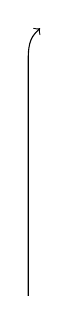
\begin{tikzpicture}[x=0.25cm,y=0.25cm]
\draw[->] (0,0)--(0,12).. controls (0,13) and (0.2,13.2)..(0.6,13.6);
\end{tikzpicture}}

D'autre part le sous-groupe de
\[
\mathcal M_{\rho,\sigma}(0)\simeq\tau_{\rho,\sigma}\subset B'_0\times T_\rho\times N'_\sigma
\]
qui opère trivialement sur $SG$, est \inserted{l'intersection de $\tau_{\rho,\sigma}$ avec} $(\deleted{\unsure{\mu_2}}\inserted{1}\times T_\rho\times N'_\sigma)$, car $B'_0$ opère \unsure{trivialt} \deleted{$\mu_2\unsure{\subset}B'_0$} (puisque
\[
(46)\qquad B'_0\cap\underbrace{\mu_2}_{\substack{\text{centre de}\\SG}}=\{1\}
\]
. C'est donc le \unsure{s-groupe} des
\[
(47)\qquad
\left\{\left(1,\underset{\in\,\Gamma T_\rho}{\underline a},\underset{\in\,\Gamma N'_\sigma}{\underline b}\right)\mid(\det\underline a)^2=1,\ \det\underline b=1\right\}
\]

\margin{\unsure{non!}}
\uline{Reste} : déterminer \uline{le centre de} $\tau_{\rho,\sigma}$, extension de $\mu_2\times\mu_2$ par $\tau^0_{\rho,\sigma}\simeq\mathcal G^*_{\rho,\sigma}(0)^0\subset T_0^0\times T_\rho\times\deleted{\unsure{N'_\sigma}}\inserted{T_\sigma}$. Comme $\tau^0_{\rho,\sigma}$ est commutatif, il suffit de déterminer l'action de $\mu_2\times\mu_2$ sur $\tau^0_{\rho,\sigma}$, et d'en déterminer le sous-groupe des invariants.
\margin{Cela donnera au moins l'intersection du centre \unsure{avec} $\tau^0_{\rho,\sigma}$.}
\margin{408}

\scanpage{410}
\mspage{506}

Notons que l'on a
\[
\tau_{\rho,\sigma}=S\mathcal G^*_{\rho,\sigma}(0)\subset\mathcal G^*_{\rho,\sigma}(0)\simeq T_0\times T_\rho\times N'_\sigma
\]
et on a un hom de suites exactes

\noindent$(48)$\quad
\diagram{\begin{tikzcd}[ampersand replacement=\&,column sep=large,row sep=large]
1\arrow[r]\&\tau^0_{\rho,\sigma}\arrow[r]\arrow[d,hook]
\&\tau_{\rho,\sigma}\arrow[r,"{(\underline u,\underline a,\underline b)\mapsto(\varepsilon(\underline b),\det\underline a/\det(\underline u))}"]\arrow[d,hook]
\&\mu_2\times\mu_2\arrow[r]\arrow[d,"{\substack{\text{première}\\\text{proj}}}"]\&1\\
1\arrow[r]\&\unsure{T_0}\times T_\rho\times\deleted{\unsure{N'_\sigma}}\inserted{T_\sigma}\arrow[r]
\&T_0\times T_\rho\times N'_\sigma\arrow[r]\&\mu_2\arrow[r]\&1
\end{tikzcd}},

qui montre que l'action de $\mu_2\times\mu_2$ sur \deleted{$\unsure{\tau}$} $\tau^0_{\rho,\sigma}$ se fait par l'intermédiaire de la projection de $\mu_2\times\mu_2$ sur son premier facteur, et ce par l'opération de celui-ci sur $T_0\times T_\rho\times T_\sigma$ qui opère trivialement sur $T_0\times T_\rho$, et qui sur $T_\sigma$ est l'opération canonique de $\mu_2$ sur $T_\sigma$, $\sigma\mapsto\varepsilon\sigma$, dont les invariants sont réduits aux scalaires $\mathbb G_m$. \deleted{Donc on trouve} \inserted{Ce raisonnement} montre, plus généralement, que la \unsure{\deleted{portion}} \inserted{du centre de $\tau_{\rho,\sigma}$} sur le sous-groupe $\tau'_{\rho,\sigma}\subset\tau_{\rho,\sigma}$ noyau de

\diagram{\begin{tikzcd}[ampersand replacement=\&,column sep=large]
\tau_{\rho,\sigma}\arrow[r]\&\mu_2\times\mu_2\arrow[r,"{\text{1\textsuperscript{ère} proj}}"]\&\mu_2\\
(\underline u,\underline a,\underline b)\arrow[rr,mapsto]\&\&\varepsilon(\underline b)
\end{tikzcd}}

est aussi la trace, sur ce sous-groupe, de $T_0\times T_\rho\times\mathbb G_m$. D'ailleurs, comme $\mu_2$ opère \uline{fidèlement} sur $T_\sigma$ via $\sigma\mapsto\varepsilon\sigma$, on voit \deleted{que} aussitôt qu'il opère aussi fidèlement sur $\tau'_{\rho,\sigma}$ (qui en effet s'envoie \uline{\unsure{épimorphiquement}} sur $T_\sigma$ !) donc on a

\diagram{\begin{tikzcd}[ampersand replacement=\&,column sep=large]
\uline{\mathrm{Centre}}(\tau_{\rho,\sigma})\subset\tau'_{\rho,\sigma}=\operatorname{Ker}\bigl(\tau_{\rho,\sigma}
\arrow[r,"{(\underline u,\underline a,\underline b)\mapsto\varepsilon(\underline b)}"]\&\mu_2\bigr)
\end{tikzcd}}
\margin{409}

\scanpage{411}

Donc en résumé
\[
(49)\quad
\left\{
\begin{array}{l}
\uline{\mathrm{Centre}}(\mathcal G^*_{\rho,\sigma}(0))=T_0\times T_\rho\times\mathbb G_m\\[5pt]
\uline{\mathrm{Centre}}\left(\underset{S\mathcal G^*_{\rho,\sigma}(0)}{\underline{\tau_{\rho,\sigma}}}\right)
=\deleted{\unsure{\mathrm{Centre}}}(T_0\times T_\rho\times\mathbb G_m)\cap\tau_{\rho,\sigma}\\[7pt]
\hspace{7em}=\left\{\left(
\underset{\substack{\in\Gamma T_0\\\simeq\Gamma\mathbb G_m}}{\underline u},
\underset{\in\Gamma T_\rho}{\underline a},
\underset{\in\Gamma\mathbb G_m}{\unsure{\lambda}}
\right)\mid u=\lambda^2,\ \deleted{\unsure{\underline a}}\inserted{\det\underline a}=\varepsilon'\unsure{\lambda^2},\ \varepsilon'^2=1\right\}
\end{array}\right.
\]

Le sous-groupe du centre qui opère \unsure{trivialt} sur $SG$ est donc, en vertu de (47), donné par la restriction suppl. $u=1$, il s'identifie donc à \deleted{$\mu_2\times\mu_2$}
\[
(50)\quad
\left\{
\begin{array}{l}
1\times\unsure{ST'_\rho}\times\mu_2\subset\tau^{\unsure{a|0}}_{\rho,\sigma}\subset T_0\times T_\rho\times\unsure{N'_\sigma}\\[5pt]
\text{où }\unsure{ST'_\rho}\subset T_\rho\\[3pt]
\hspace{3em}\wr\ \{\underline a\mid(\det\underline a)^2=1\}
\end{array}\right.
\]

Donc
\[
(51)\quad
\deleted{\uline{\mathrm{Centr}}(\mathcal M_{\rho,\sigma})\simeq
\left(\underset{\in T_0}{1}\times\unsure{ST'_\rho}\times\underset{\in T_\sigma}{\mu_2}\right)\times\underset{\in SG}{\mu_2}}
\]
\margin{\uline{faux} le centre est plus grand,}

Le groupe des points entiers de ce \deleted{centre}\inserted{groupe}, dans le cas modulaire, est réduit :
\[
(52)\quad
\left\{
\begin{array}{l}
\mathbb Z/6\mathbb Z\times\mathbb Z/2\mathbb Z\times\mathbb Z/2\mathbb Z\\[4pt]
\simeq\mathbb Z/3\mathbb Z\times(\mathbb Z/2\mathbb Z\times\mathbb Z/2\mathbb Z\times\mathbb Z/2\mathbb Z),
\end{array}\right.
\]
\deleted{\unsure{Groupe de}}
\margin{\uline{NB} Ce groupe est en fait contenu dans $\mathcal M^0_{\rho,\sigma}(\mathbb Z)$.}

produit d'un groupe cyclique d'ordre $3$ (engendré naturellement par $-\rho$) par un groupe $(\mathbb Z/2\mathbb Z)^3$, qui n'est autre que le groupe $\Sigma$ déjà dans (\uline{IX}).

Plus intéressant serait sans doute le
\margin{410}

\scanpage{412}
\mspage{507}

centre de $\mathcal{M}_{\rho,\sigma}^{\circ}$, qui sera donc le produit direct du centre \inserted{$\mu_2$} de $SG$ (sur lequel le groupe \inserted{\uline{commutatif}} $\mathcal{M}_{\rho,\sigma}^{\circ}(0)\simeq\tau_{\rho,\sigma}^{\circ}$ opère \unsure{trivialement}) par le ss-groupe de $\tau_{\rho,\sigma}^{\circ}\subset T_0\times T_\rho\times T_\sigma$ qui opère \unsure{trivialement} sur $SG$, savoir \deleted{$\unsure{\tau_{\rho,\sigma}}$}

\margin{\uline{faux}}

\[
\begin{aligned}
\tau_{\rho,\sigma}^{\circ}\cap 1\times T_\rho\times\unsure{T_\sigma}
 &=\{(1,\uline{a},\uline{b})\mid\det\uline{b}=1,\,
 \deleted{(}\det\uline{a}\deleted{)^{\unsure{2}}}=1\}\\
 &\simeq ST_\rho\times ST.
\end{aligned}
\]
\margin{(et pas seulement $(\det a)^2=1$, car on est dans $\tau_{\rho,\sigma}^{\circ}$}

Donc

\unsure{On}
\deleted{\diagram{\[\begin{array}{rcl}
(53)\quad\uline{\mathrm{Centre}}(\mathcal{M}_{\rho,\sigma}^{\circ})
 &=&(1\times ST_\rho\times ST_\sigma)\times\mu_2\quad,\\
 &&\hfill\cap\qquad\\[-2pt]
 &&\hfill SG\qquad
\end{array}\]}}

\margin{\uline{faux} ! Centre \unsure{est} de dim 3}

donc dans le cas modulaire on a

\deleted{\diagram{\[\begin{array}{rclccccccc}
(\unsure{54|14})\quad\uline{\mathrm{Centre}}(\mathcal{M}_{\rho,\sigma}^{\circ})(\mathbb Z)
 &\simeq&1&\times&\mathbb Z/6\mathbb Z&\times&\mathbb Z/4\mathbb Z&\times&\mathbb Z/2\mathbb Z\\
 &&&&\Vert&&\Vert&&\Vert\\
 &&&&\Gamma(ST_\rho)&&\Gamma(ST_\sigma)&&\Gamma\mu_2\subset\Gamma(SG)
\end{array}\]}}

\deleted{qui n'est que deux fois plus gros que \deleted{$\unsure{\mathcal{M}_{\rho,\sigma}}$} le groupe des pts entiers du centre de $\mathcal{M}_{\rho,\sigma}$. \deleted{(\unsure{bien que celui-ci}}}

\deleted{\uline{Rmq.} La composante neutre du centre de $\mathcal{M}_{\rho,\sigma}^{\circ}$ est bien sûr $ST_\rho\times ST_\sigma$, comme le suggérait le \unsure{dévissage|discussion} du th. p. $501'$.}

\margin{411}

\scanpage{413}
\mspage{508}

\uline{$\overline{\mathrm{XI}}$}\quad\uline{Récapitulation sur le groupe} $\mathcal{M}_{\rho,\sigma}$.

\margin{\uline{Préliminaires}}

\textcircled{$1^\circ$} Étant donné, sur un schéma $S$, une forme $G$ de $\mathrm{Gl}(2)$, d'où des formes $SG$, $PG$ de $\mathrm{Sl}(2)$, $\unsure{\mathrm{GP}(1)|\mathrm{PGl}(1)}$, et deux sections $\widetilde\rho,\widetilde\sigma$ de $PG$, et un sous-groupe à \unsure{1-paramètre} \deleted{\unsure{multiplicatif|complet}} additif \unsure{bordé|basé}
\diagram{\begin{tikzcd}[ampersand replacement=\&,column sep=large]
\widetilde{\uline{\unsure{\xi|\varepsilon}}}_0:\ G_a \arrow[r,hook] \& PG
\end{tikzcd}}
\inserted{$\unsure{\xi_0|\varepsilon_0}$}
(ce qui revient au $\overline{\mathrm m}$, une section \deleted{\unsure{de}} unipotente régulière \unsure{de} $\unsure{\xi_0|\varepsilon_0}$ de $G$, ou une section nilpotente régulière $N_0$ dans la forme $\mathcal M$ de $\mathrm{M}_2(\mathcal O_S)$ associée à $G$) --- satisfaisant les conditions
\[
\begin{aligned}
(1)\quad &\widetilde\sigma^{-1}\widetilde\rho
  =\widetilde{\uline{\unsure{\xi|\varepsilon}}}_0(1),\qquad
  \widetilde{\uline{\unsure{\xi|\varepsilon}}}_0\text{ et }
  \widetilde{\uline{\unsure{\xi|\varepsilon}}}_1
  =\rho\bigl(\widetilde{\uline{\unsure{\xi|\varepsilon}}}_0\bigr)
  \bigl(=\sigma\bigl(\widetilde{\uline{\unsure{\xi|\varepsilon}}}_0\bigr)\bigr)
  \text{ sont}\\
 &\hspace{10em}\text{indépendants sur chaque fibre}\\[4pt]
(2)\quad &\mathrm{Tr}\,\sigma=0\qquad
 \text{si }\sigma\text{ est un relèvement local de }\widetilde\sigma,
\end{aligned}
\]

On définit des relèvements \uline{canoniques} $\rho$, $\sigma$ de $\widetilde\rho,\widetilde\sigma$ à $G$, \deleted{\unsure{satisfais}} par les conditions
\[
(3)\quad\deleted{\unsure{\sigma\rho}}
\left\{\begin{array}{ll}
 \unsure{\xi_0|\varepsilon_0}=-\sigma^{-1}\rho
 &\text{i.e. }\unsure{\xi_1|\varepsilon_1}=-\rho\sigma^{-1}\\
 \mathrm{Tr}(\rho+\sigma)=1
 &\text{i.e. }\mathrm{Tr}\,\rho=1,
\end{array}\right.
\]
et les constructions qui suivent ont un sens.

On construit un \unsure{épinglage}
\diagram{\begin{tikzcd}[ampersand replacement=\&,column sep=large]
\deleted{(\unsure{4})}\ (5)\quad\deleted{\unsure{\tau_{\rho,\sigma}}=}\ \mathrm{Gl}(2)
 \arrow[r,"\sim"] \& G
\end{tikzcd}}
par la condition que $\unsure{\xi_1|\varepsilon_1}$ prenne la forme
\[
(6)\qquad\unsure{\xi_1|\varepsilon_1}
 =\begin{pmatrix}1&0\\1&1\end{pmatrix}
\]
d'où
\[
(7)\quad\left\{\begin{array}{l}
\displaystyle\rho=\begin{pmatrix}0&1\\\unsure{v|\upsilon}&1\end{pmatrix},\qquad
 \sigma=\begin{pmatrix}0&-1\\-\unsure{v|\upsilon}&0\end{pmatrix}
 \qquad(\unsure{v|\upsilon}\in\Gamma G_m\\[6pt]
\det\rho=\det\sigma=-\unsure{v|\upsilon}
\end{array}\right.
\]
\[
(8)\qquad\unsure{\xi_0|\varepsilon_0}
 =\begin{pmatrix}1&1/\unsure{v|\upsilon}\\0&1\end{pmatrix},
\]

\margin{412}

\scanpage{414}

on considère les sous-groupes
\[
(9)\quad\left\{\begin{array}{ll}
 L_0=\{\uline{\unsure{\xi|\varepsilon}}_0(\lambda)\}
   =\left\{\begin{pmatrix}1&\lambda\\0&1\end{pmatrix}\right\}
 & (\lambda\in\Gamma G_a)\\[7pt]
 L_1=\sigma(L_0)=\rho(L_0)
   =\{\uline{\unsure{\xi|\varepsilon}}_1(\lambda)\}
   =\left\{\begin{pmatrix}1&0\\\lambda&1\end{pmatrix}\right\}
 & \backslash\;\unsure{\text{id}}\\[7pt]
 B'_0=\left\{\begin{pmatrix}\mu&\lambda\\0&1\end{pmatrix}
       \mid\mu\in\Gamma G_m,\,\lambda\in\Gamma G_a\right\} &\\[7pt]
 T_0=\left\{\begin{pmatrix}\mu&0\\0&1\end{pmatrix}
       \mid\mu\in\Gamma G_m\right\} &
\end{array}\right.
\]
d'où
\[
(10)\qquad B'_0=T_0.L_0\qquad\text{(produit $\frac12$-direct)}
\]
\margin{\unsure{---}}

et on a des iso
\diagram{\[
(11)\quad\left\{\begin{gathered}
\begin{tikzcd}[ampersand replacement=\&,column sep=large,row sep=large]
\uline{\unsure{\xi|\varepsilon}}_0:\ G_a \arrow[r,"\sim"] \& L_0
 \&\lambda\arrow[r] \&\unsure{\xi_0|\varepsilon_0}(\lambda)
      =\begin{pmatrix}1&\lambda/\unsure{v|\upsilon}\\0&1\end{pmatrix}\\
\uline{\unsure{\xi|\varepsilon}}_1:\ G_a \arrow[r,"\sim"] \& L_1
 \&\lambda\arrow[r] \&\unsure{\xi_1|\varepsilon_1}(\lambda)
      =\begin{pmatrix}1&0\\\lambda&1\end{pmatrix}
\end{tikzcd}\\[5pt]
\text{donc }\uline{\unsure{\xi|\varepsilon}}_1(\lambda)
  =\rho\unsure{(\,|\{\,}\unsure{\xi_0|\varepsilon_0}(\lambda))
  =\sigma(\unsure{\xi_0|\varepsilon_0}(\lambda)).
\end{gathered}\right.
\]}

On \deleted{pose} considère
\[
(12)\quad\deleted{\unsure{\mathcal{G}_{\rho,\sigma}}}
\left\{\begin{aligned}
 T_\rho&=\text{schém. des unités de }\mathcal A_\rho
  =\uline{\mathcal O}_S+\uline{\mathcal O}_S\rho\\
 &\hspace{17em}\simeq\uline{\mathcal O}_S[X]/(X^2-X-\unsure{v|\upsilon})\\
 &\deleted{\text{\unsure{de}}\ \uline{\mathcal O}_S}\\
 T_\sigma&=\text{schém. des unités de }\mathcal A_\sigma
  =\uline{\mathcal O}_S+\uline{\mathcal O}_S\sigma\\
 &\hspace{17em}\simeq\uline{\mathcal O}_S[Y]/(Y^2-\unsure{v|\upsilon})
\end{aligned}\right.
\]
\diagram{\[\begin{array}{rcl}
(13)\quad &N'_\sigma&=\{g\in\Gamma G\mid g(\sigma)=\varepsilon\sigma,\ \varepsilon^2=1\}\\
 &\cap&\\[-2pt]
 &G&
\end{array}\]}
d'où
\diagram{\begin{tikzcd}[ampersand replacement=\&,column sep=large]
(14)\quad 1\arrow[r] \&T_\sigma\arrow[r] \&N'_\sigma\arrow[r,"\varepsilon_\sigma"] \&\mu_2\arrow[r] \&1.
\end{tikzcd}}

On pose
\[
(15)\quad\left\{\begin{aligned}
 \mathcal{G}_{\rho,\sigma}&=B'_0\times T_\rho\times T_\sigma\\[4pt]
 \mathcal{G}_{\rho,\sigma}^{*}&=B'_0\times T_\rho\times N'_\sigma.
\end{aligned}\right.
\]

\margin{413}

\scanpage{415}
\mspage{509}

\margin{$\begin{gathered}
 \mathcal M_{\rho,\sigma}[0],\ \mathcal M_{\rho,\sigma}(0)\,,\\
 \unsure{\tau_{\rho,\sigma}|\mathcal G_{\rho,\sigma}},\ \tau_{\rho,\sigma}^{\circ}\,,\\
 \mathcal M_{\rho,\sigma},\ \widetilde{\mathcal G}_{\rho,\sigma}^{+}\quad
   \deleted{\unsure{\mathcal M_{\rho,\sigma}^{\circ}}}\\
 \tau_{\rho,\sigma}^{\circ\unsure{+|*}}
\end{gathered}$}

\textcircled{$2^\circ$} On introduit
\[
\begin{aligned}
(16)\quad \mathcal M_{\rho,\sigma}[0]
 &\subset \unsure{\mathcal B_{\rho,\sigma}^{*}|\mathcal G_{\rho,\sigma}^{*}}
   =B'_0\times T_\rho\times N'_\sigma\\
 &\mathrel{\mathop{=}\limits^{\mathrm{dfn}}}
 \{(\uline u,\uline a,\uline b)\mid
   \det\uline u=\det\uline b=\varepsilon'\det\uline a,\
   \varepsilon'{}^2=1\}
\end{aligned}
\]
\[
(17)\qquad \mathcal M_{\rho,\sigma}(0)\subset\mathcal M_{\rho,\sigma}[0]
 \qquad\text{défini par }\uline u=1\quad\text{i.e.}
\]
\[
 \mathcal M_{\rho,\sigma}(0)=\mathcal M_{\rho,\sigma}[0]
   \cap(T_0\times T_\rho\times N'_\sigma)
 \qquad\text{dans }\mathcal G_{\rho,\sigma}^{*}.
\]
\diagram{\begin{tikzcd}[ampersand replacement=\&,column sep=large,row sep=small]
(18)\quad L_0\arrow[r,hook] \&\mathcal M_{\rho,\sigma}[0]\\
\lambda\arrow[r,mapsto] \&(\lambda,1,1)
\end{tikzcd}}
donc on a
\[
(19)\qquad \mathcal M_{\rho,\sigma}[0]\simeq
  \mathcal M_{\rho,\sigma}\unsure{[0)|(0)}\, .\, L_0
 \qquad\text{produit }\tfrac12\text{-direct}
\]

On a un homomorphisme
\diagram{\begin{tikzcd}[ampersand replacement=\&,column sep=huge]
(20)\quad\unsure{\dot{\mathcal M}|\mathcal M}_{\rho,\sigma}[0]\arrow[r]
 \&G_m\times\mu_2\times\mu_2
\end{tikzcd}}
\[
 \text{noté }\{g\mapsto\chi(g),\varepsilon_2(g),\varepsilon_3(g)
\]
pour $g=(\uline u,\uline a,\uline b)$ on a
\[
\begin{aligned}
 \chi(g)&=\det\uline u=\det\uline b\\
 \varepsilon_2(g)&=\varepsilon_\sigma(b)\qquad\text{(cf (13)(14)}\\
 \varepsilon_3(g)&=\det(\uline a)/\det\uline b\\
 &\text{i.e. }\left\{\begin{array}{l}
    \det a=\varepsilon_3\mu\\
    \text{où }\mu=\chi(g)
  \end{array}\right.
\end{aligned}
\]
trivial sur $L_0$ (donc se factorisant par le quotient). On pose aussi
\[
(21)\qquad\tau_{\rho,\sigma}\simeq\mathcal M_{\rho,\sigma}[0]/L_0
 \qquad\text{\unsure{où}}
\]
\margin{Cette notation n'est pas du tout adéquate (\unsure{inspirée à tort} du $\tau_{g,\unsure{\nu|r}}$) \unsure{la suite montre} (et ce qui précède montrait déjà) que la notation $\Gamma_{\rho,\sigma}$ conviendrait, inspirée par $\Gamma_{g,\nu}$ et $\Gamma_{0,3}$.}

\unsure{et} le composé
\diagram{\begin{tikzcd}[ampersand replacement=\&,column sep=large]
(22)\quad\mathcal M_{\rho,\sigma}(0)\arrow[r,hook]
 \&\mathcal M_{\rho,\sigma}[0]\arrow[r] \&\tau_{\rho,\sigma}
\end{tikzcd}}
est un \uline{iso}, d'où on a
\diagram{\begin{tikzcd}[ampersand replacement=\&,column sep=large]
(23)\quad\unsure{\mathcal M|\mathcal G}_{\rho,\sigma}(0)
 \simeq\unsure{\tau_{\rho,\sigma}|\tau_{\rho,\sigma}'}\arrow[r,hook]
 \&T_0\times T_\rho\times N'_\sigma
\end{tikzcd}}

\margin{414}
